
\chapter{ZU ÜBERARBEITEN}


\subsection{Gesamtes Modell}
\todo{erklärung Anschlusspunkt}
\begin{center}
$max_{X^{in}_{RL}(s_{RL}), X^{out}_{RL}(s_{RL}), X_{DA}(s_{DA}), X^{in}_{RA}(s_{RA}), X^{out}_{RA}(s_{RA})} Profit $\\
$=$\\
        $\sum_{s^{in}_{RL}} X^{in}_{RL}(s_{RL}) * p(s^{in}_{RL}) * \omega_{RL}(s^{in}_{RL}) +$\\
        $\sum_{s^{out}_{RL}} X^{out}_{RL}(s_{RL}) * p(s^{out}_{RL}) * \omega_{RL}(s^{out}_{RL}) +$\\
        $\sum_{s_{DA}} X_{DA}(s_{DA}) * p(s_{DA}) * \omega_{DA}(s_{DA}) +$\\
	$\sum_{s^{in}_{RA}} Q^{in}_{RA}(s_{RA}) * p(s^{in}_{RA}) * \omega_{RA}(s^{in}_{RA}) +$\\
	$\sum_{s^{out}_{RA}} Q^{out}_{RA}(s_{RA}) * p(s^{out}_{RA}) * \omega_{RA}(s^{out}_{RA})$\\
\end{center}
s.t.:\\
(Anschlusspunkt)\\
        $a + X^{in}_{RA}(s^{in}_{RA}) \geq X_{DA}(s_{DA}) + X^{out}_{RA}(s^{out}_{RA}) \quad\forall s^{in}_{RL},s^{in}_{RA}),s^{out}_{RL},s^{out}_{DA},s^{out}_{RA} $\\
(min. $RA \geq RL$)\\
        $ X^{in}_{RA} * B^{in}_{RL}(s^{in}_{RA}) \geq X^{in}_{RL} * B^{in}_{RL}(s^{in}_{RL})$\\
        $ X^{out}_{RA} * B^{out}_{RL}(s^{out}_{RA}) \geq X^{out}_{RL} * B^{out}_{RL}(s^{out}_{RL})$\\
RL\\
        (für binäre Zuschlagsvariable:)\\
        $c^{in}_{RL} \leq p^{in}(s^{in}_{RL}) + M * B^{in}_{RL}(s^{in}_{RL})\quad\forall s^{in}_{RL} $ \\
        $c^{in}_{RL} \geq p^{in}(s^{in}_{RL}) - M * (1 - B^{in}_{RL}(s^{in}_{RL}))\quad\forall s^{in}_{RL} $ \\
        $c^{out}_{RL} \leq p^{out}(s^{out}_{RL}) + M * B^{out}_{RL}(s^{out}_{RL})\quad\forall s^{out}_{RL} $ \\
        $c^{out}_{RL} \geq p^{out}(s^{out}_{RL}) - M * (1 - B^{out}_{RL}(s^{out}_{RL}))\quad\forall s^{out}_{RL}$  \\
        (für linearität der Mengenvariable:)\\
        $X^{in}_{RL}(s^{in}_{RL}) \leq B^{in}_{RL}(s^{in}_{RL}) * r \quad\forall s^{in}_{RL}$\\
        $Q^{in}_{RL}(s_{RL}) - X^{in}(s_{RL}) \leq (1 - B^{in}_{RL}(s_{RL})) * r \quad\forall s^{in}_{RL}$\\
        $Q^{in}_{RL}(s_{RL}) - X^{in}(s_{RL}) \geq 0 \quad\forall s^{in}_{RL}$\\
        $X^{out}_{RL}(s^{out}_{RL}) \leq B^{out}_{RL}(s^{out}_{RL}) * r \quad\forall s^{out}_{RL}$\\
        $Q^{out}_{RL}(s_{RL}) - X^{out}_{RL}(s_{RL}) \leq (1 - B^{out}(s_{RL})) * r \quad\forall s^{out}_{RL}$\\
        $Q^{out}_{RL}(s_{RL}) - X^{out}_{RL}(s_{RL}) \geq 0\quad\forall s^{out}_{RL} $\\
        (grundlegende Beschränkungen der Definitionsbereiche:)\\
        $B^{in}_{RL}(s^{in}_{RL}),B^{out}_{RL}(s^{out}_{RL}) \in \{0,1\}\quad\forall s^{in}_{RL},s^{out}_{RL} $\\
        $X^{in}_{RL}(s^{in}_{RL}),X^{out}_{RL}(s^{out}_{RL}) \geq 0 \quad\forall s^{in}_{RL},s^{out}_{RL} $\\
        $Q^{in}_{RL}(s^{in}_{RL}),Q^{out}_{RL}(s^{out}_{RL}) \geq 0\quad\forall  s^{in}_{RL},s^{out}_{RL} $\\
DA\\
        (für binäre Zuschlagsvariable:)\\
        $c_{DA} \leq p(s_{DA}) + M * B_{DA}(s_{DA})\quad\forall s_{DA} $ \\
        $c_{DA} \geq p(s_{DA}) - M * (1 - B_{DA}(s_{DA}))\quad\forall s_{DA} $ \\
        (für linearität der Mengenvariable:)\\
        $X_{DA}(s_{DA}) \leq B_{DA}(s_{DA}) * r \quad\forall s_{DA}$\\
        $Q_{DA}(s_{DA}) - X(s_{DA}) \leq (1 - B_{DA}(s_{DA})) * r \quad\forall s_{DA}$\\
        $Q_{DA}(s_{DA}) - X(s_{DA}) \geq 0 \quad\forall s_{DA}$\\
        (grundlegende Beschränkungen der Definitionsbereiche:)\\
        $B_{DA}(s_{DA})\in \{0,1\}\quad\forall s_{DA} $\\
        $X_{DA}(s_{DA}) \geq 0 \quad\forall s_{DA} $\\
        $Q_{DA}(s_{DA}) \geq 0\quad\forall  s_{DA} $\\
RA\\
	(grundlegende Beschränkungen der Definitionsbereiche:)
	$Q^{in}_{RA}(s^{in}_{RA}),Q^{out}_{RA}(s^{out}_{RA}) \geq 0 \quad\forall s^{in}_{RA},s^{out}_{RA} $\\
	$Q^{in}_{RA}(s^{in}_{RA}),Q^{out}_{RA}(s^{out}_{RA}) \geq 0\quad\forall  s^{in}_{RA},s^{out}_{RA} $\\



\subsection{Variables - simplified model}
\textbf{Vereinfachungen:}



\begin{itemize}
    \item angenommene Gebote werden auch in voller Höhe abgerufen
    \item 
\end{itemize}

asdf


asdf


asdf


asdf
\subsection{Umwandlung Linearität}
Die Kombination von $Q_{RL}(s_{RL}) * B_{RL}(s_{RL})$ würde zu einem nicht linearen Problem führen. Diese sind schwerer zu berechnen als lineare Problemstellungen. Um dies zu vermeiden wird die Kombination in eine kontinuierliche Variable $X(s_{RL})$ umgewandelt. Diese Ersatzvariable wird anschließend, mit Hilfe von 3 Nebenbedingungen, auf den Lösungsraum der ursprünglichen binär Kombination beschränkt.

\textbf{Nebenbedingungen für die binär Kombination Umwandlung}
\begin{enumerate}
    \item $X_{RL}(s_{RL}) \leq B_{RL}(s_{RL}) * r$
    \item $Q_{RL}(s_{RL}) - X_{RL}(s_{RL}) \leq (1 - B_{RL}(s_{RL})) * r $
    \item $Q_{RL}(s_{RL}) - X_{RL}(s_{RL}) \geq 0 $
\end{enumerate}
($r$ ist die Rate mit der der Speicher sich laden bzw. entladen kann)\\
Aus den Nebenbedingungen folt:\\

$X_{RL}(s_{RL}) = B_{RL}(s_{RL}) * Q_{RL}(s_{RL}) $

(für linearität der Mengenvariable:)\\
$X^{in}_{RL}(s^{in}_{RL}) \leq B^{in}_{RL}(s^{in}_{RL}) * r \quad\forall s^{in}_{RL}$\\
$Q^{in}_{RL}(s_{RL}) - X^{in}(s_{RL}) \leq (1 - B^{in}_{RL}(s_{RL})) * r \quad\forall s^{in}_{RL}$\\
$Q^{in}_{RL}(s_{RL}) - X^{in}(s_{RL}) \geq 0 \quad\forall s^{in}_{RL}$\\
$X^{out}_{RL}(s^{out}_{RL}) \leq B^{out}_{RL}(s^{out}_{RL}) * r \quad\forall s^{out}_{RL}$\\
$Q^{out}_{RL}(s_{RL}) - X^{out}_{RL}(s_{RL}) \leq (1 - B^{out}(s_{RL})) * r \quad\forall s^{out}_{RL}$\\
$Q^{out}_{RL}(s_{RL}) - X^{out}_{RL}(s_{RL}) \geq 0\quad\forall s^{out}_{RL} $\\





\subsection{Variables - extended model + wind park}
\subsubsection{Aktivierung/Deaktivierung verschiedener Szenariobaumteilstränge}
 Innerhalb einer stochastischen Programmierung wird ein Szenariobaum erstellt. Die Knoten stellen dabei Entscheidungen dar und die Äste bilden verschiedene mögliche Ausgänge ab. In unserem Fall können wir aktiv bestimmte Teile des Szenariobaums aktivieren bzw. deaktivieren.\\

\textbf{Beispiel: Day Ahead Markt}\\
Mit der Entscheidung am Day Ahead Markt teil zu nehmen aktivieren wir den Teil des Szenariobaums für den Day Ahead Markt. Anschließend wird selbstständig die Entscheidung getroffen zu welchem Preis und zu welcher Menge am Day Ahead Markt geboten werden soll. Auch die Preis- bzw. Mengenentscheidung aktivieren bestimmte Teile des Szenariobaums, die anderen nicht gewählten Pfade werden automatisch deaktiviert. Nachdem eine Gebotsabgabe erfolgt ist, ist die Annahme eines solchen Gebots ein zufallbedingtes Ereignis.

Illustriet stellt sich dann das Ganze dann wie folgt dar:
\begin{figure}[H]
    \centering
    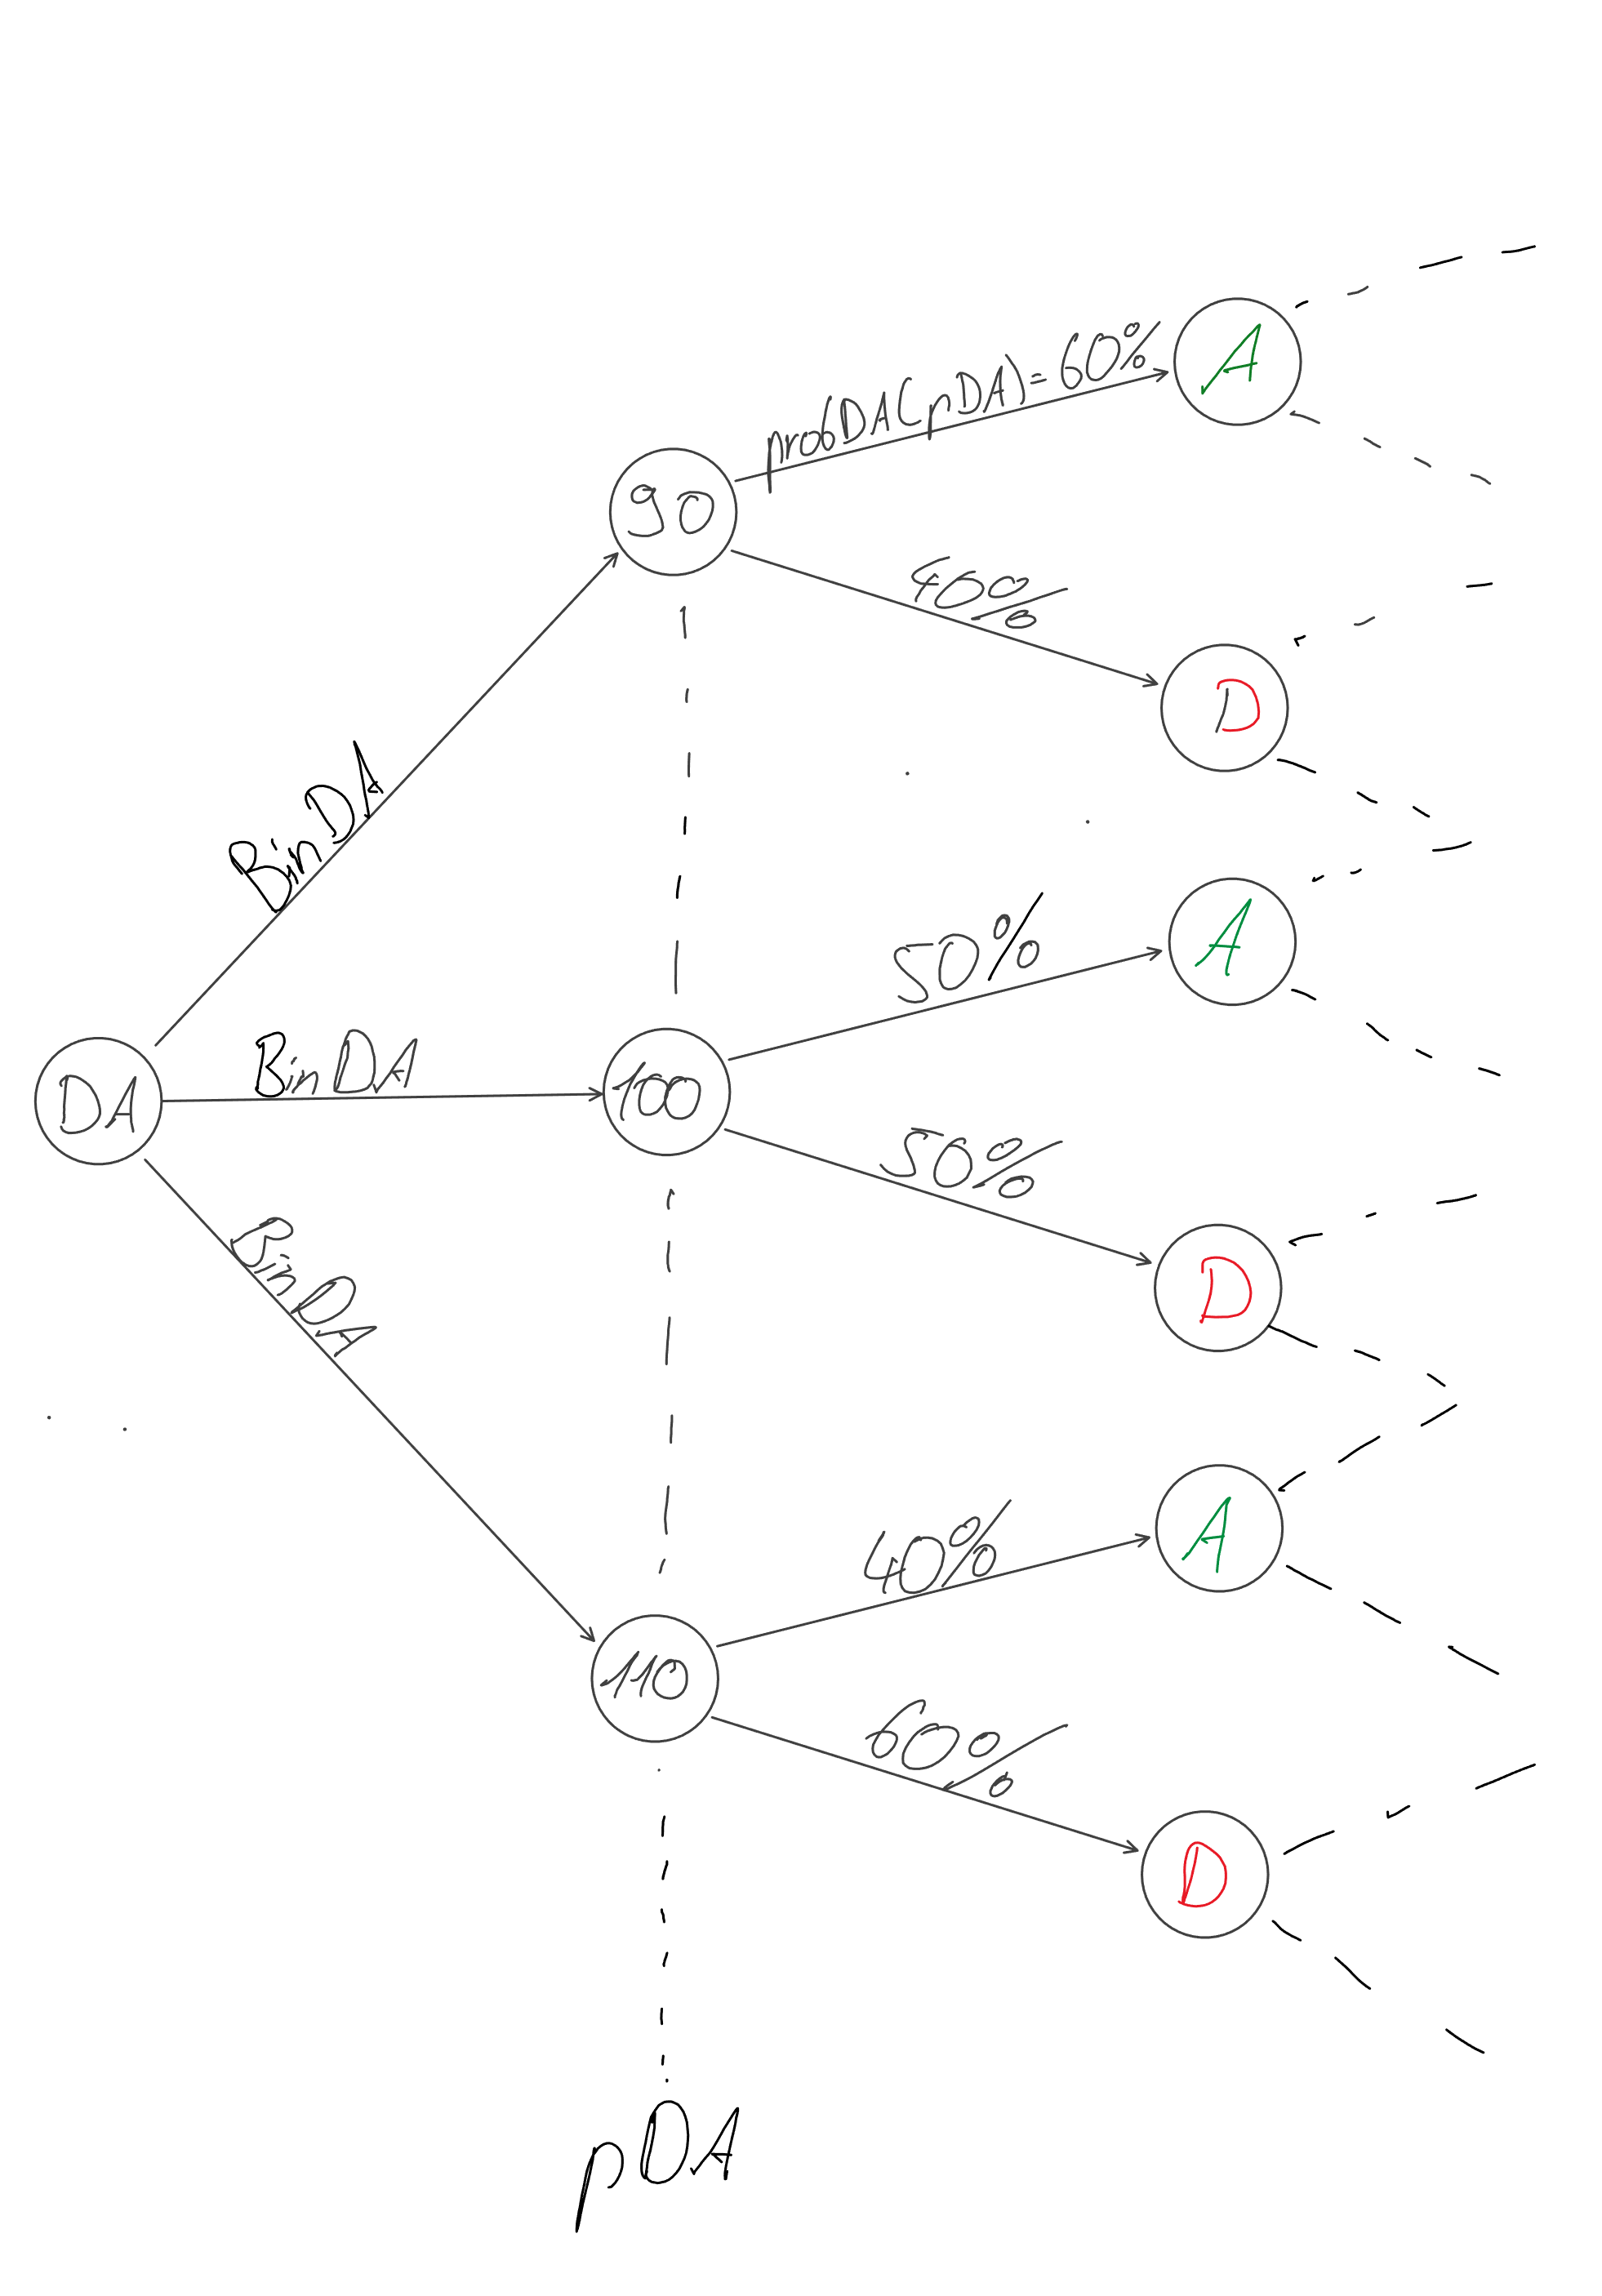
\includegraphics[width=1\linewidth]{pictures/szBaumBeispiel1.png}
    \caption{Beispielhafter Szenariobaum}
    \label{fig:enter-label}
\end{figure}
\todo{grafik neu machen mit tikz und BinDA entfernen}
Zu sehen ist ein Teil des Szenariobaums. Zur Vereinfachung ist in der Abbildung die Mengenentscheidung und die Entscheidung nicht am Day Ahead Markt teil zu nehmen ausgelassen. Zu sehen ist, dass zu verschiedenen Preisen am Day Ahead Markt geboten werden kann. 
Wird eine Entscheidung für einen Preis getroffen fallen entsprechend die anderen Teile des Szenariobaums weg.
Die anschließende Wahrscheinlichkeitsverteilung für ein aktzeptieren des Gebots ist abhängig von der Gebotshöhe aber zufällig.
In der folgenden Abbildung ist beispielhaft die Entscheidung für einen Preis von 90 grün markiert. Die entfallenden anderen Baumabschnitte sind rot markiert.\\

\begin{figure}[H]

    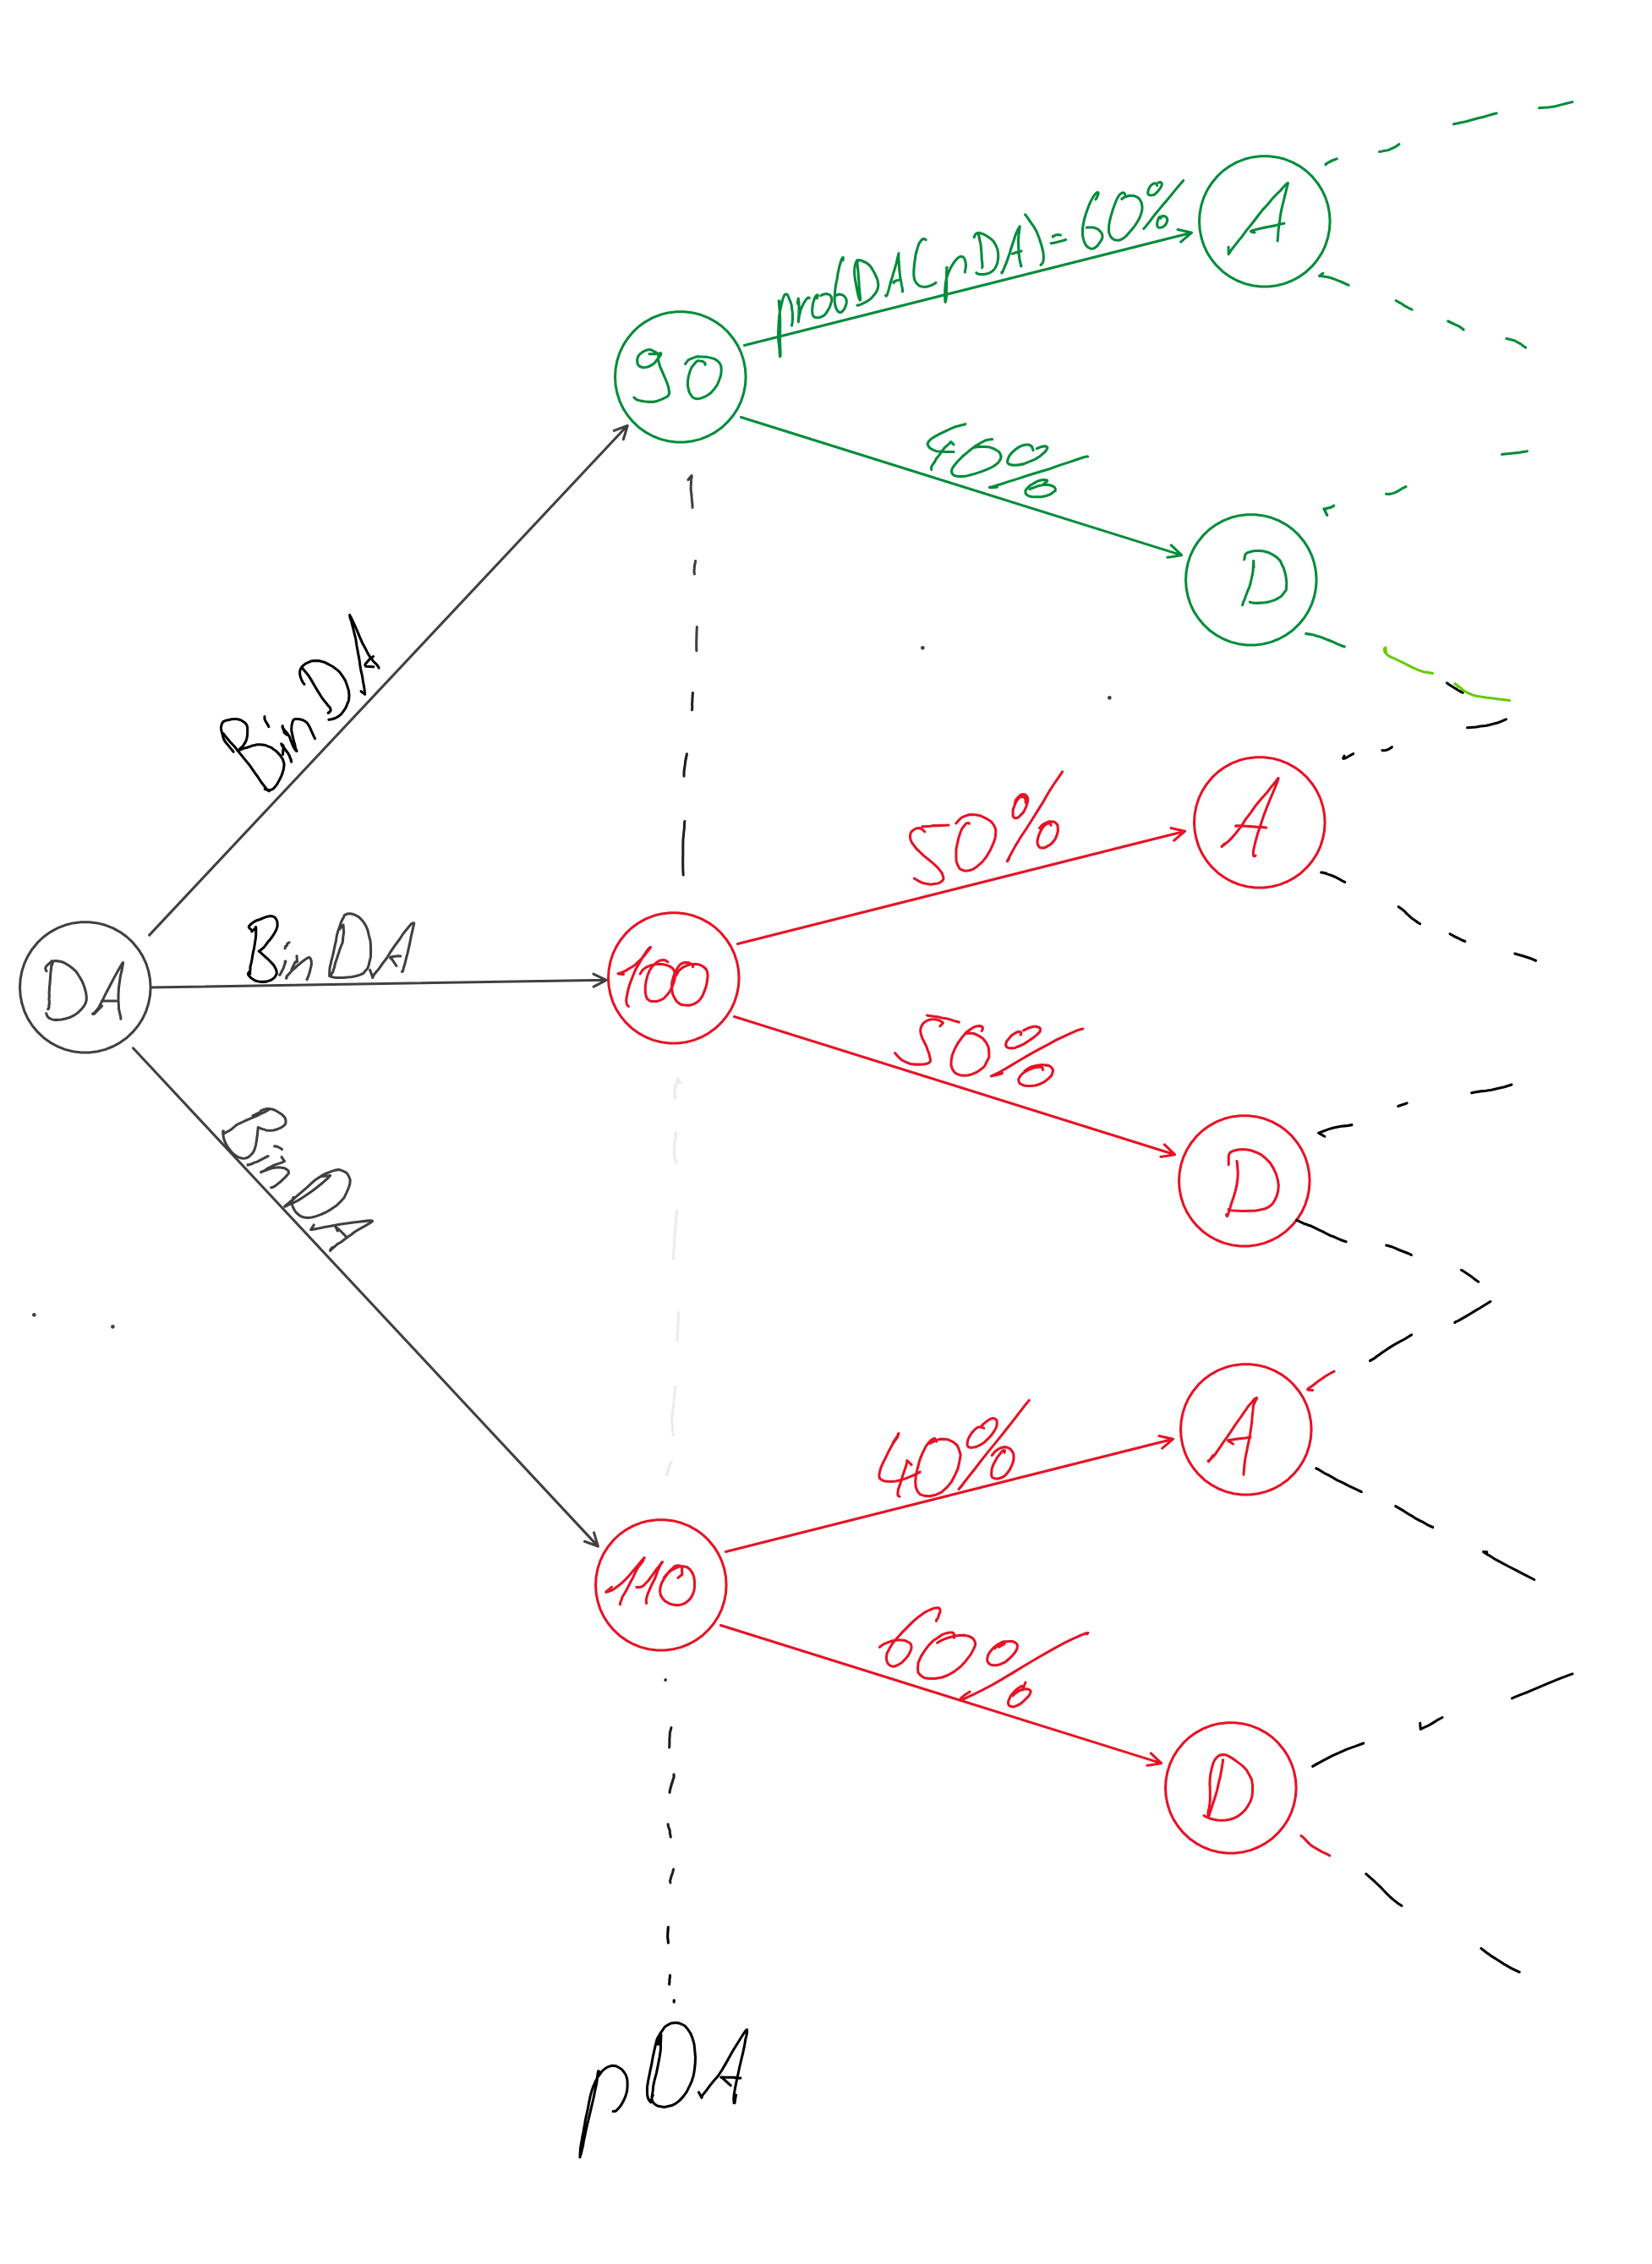
\includegraphics[width=1\linewidth]{pictures/szBaumBeispiel_markiert.png}
    \caption{Beispielhafter Szenariobaum mit markierter Entscheidung}
    \label{fig:enter-label}
\end{figure}
\todo{grafik neu machen mit tikz und BinDA entfernen}

Die Wahrscheinlichkeiten in den aktivierten Teilbäumen addieren sich zu 1 auf.
Anschließend würden sich die folgenden Märkte abbilden (hier mit gestrichelten Linien dargestellt).\\

\subsubsection{Von Umwandlung in lineares Problem}
Bisher erfolgte eine Betrachtung mit dem besonderen Augenmerk auf die Preiswahrscheinlichkeit-Kombination.
Im folgenden wird der Ausdruck $Q_{DA}$ besonders analysiert. Zunächst wird eine weitere binäre Variable eingefügt die signalisiert ob der Abruf der bereitgestellten Leistung wirklich erfolgt.
Hierraus ergibt sich:

    $B^Q_{DA} * Q_{DA}$ 

Da dieser Ausdruck zu einem nicht linearen gemischten ganzzahligen Problem führt ist es sinnvoll dieses in ein lineares Problem umzuwandeln  um die Berechenbarkeit zu verbesseren.
Dies erfolgt über eine Dummy Variable $X_{DA}$. Die Dummy Variable wird anschließend so restriktiert, dass sie sich wie $B^Q_{DA} * Q_{DA}$ verhält.
\\
Nebenbedingungen:\\
$X_{DA} \leq B^Q_{DA} * R$\\
$Q_{DA} - X_{DA} \geq (1 - B^Q_{DA}) * R$\\
$Q_{DA} - X_{DA} \geq 0 $\\
Aus den Nebenbedingung folgt entsprechend:\\
$X_{DA} = B^Q_{DA} * Q_{DA}$\\

So wird aus dem nicht linearen Problem\\
$Ertrag_{DA} = B^Q_{DA} * Q_{DA} * \sum_{s_{DA}}  p_{DA}(s_{DA}) * \omega_{DA}(s_{DA})  $\\
Das lineare Problem\\
$Ertrag_{DA} = X_{DA} * \sum_{s_{DA}} * p_{DA}(s_{DA}) * \omega_{DA}(s_{DA})  $\\
s.t.:\\
$\sum_{s_{DA}} = 1$\\
$X_{DA} \leq B^Q_{DA} * R$\\
$Q_{DA} - X_{DA} \geq (1 - B^Q_{DA}) * R$\\
$Q_{DA} - X_{DA} \geq 0 $\\


$Ertrag_{L} = B^Q_{L} * Q_{L} * \sum_{s_{L}} B^P_{L}(s_{L}) * p_{L}(s_{L}) * \omega_{L}(s_{L})  $\\ 


\subsection{Data}
Cause we want to have every number to be reduced when scaling by 10\%.
But if we simply multiply -10 with 10\% it actually gets bigger